\documentclass{beamer}

\usepackage[utf8]{inputenc}% -> pour les accents
\usepackage[T1]{fontenc}
%\usepackage[a4paper,left=3cm,right=3cm,top=3cm,bottom=3cm]{geometry}
\usepackage[english]{babel} % -> en francais
\usepackage{amsmath} % -> symboles mathématiques. amsmath inclut d'autres packages pour écrire en math comme amssymb,amstext, ...
\usepackage{hhline}% -> package supplémentaire permettant le double soulignement
\usepackage{amsfonts}
\usepackage{amssymb}
\usepackage{graphicx} % -> pour pouvoir mettre des dessins

\usepackage[toc,page]{appendix}
\usepackage{url}
\usepackage{color}
\usepackage{shadow}
\usepackage{fancybox}
\usepackage[babel=true]{csquotes}
\usepackage{bigfoot} % pour utiliser \verb dans une footnote
\usepackage{bm}

\def\N{\mathbb{N}}
\def\R{\mathbb{R}}
\def\Q{\mathbb{Q}}
\def\Z{\mathbb{Z}}
\def\C{\mathbb{C}}

\author{Cédric Simal}
\date{\today}
\title{Do you believe in Real numbers?}


\usetheme{Boxes}

\setbeamertemplate{navigation symbols}{
	\hspace{1em} \usebeamerfont{footline} \insertframenumber/\inserttotalframenumber }

\begin{document}

\frame{\titlepage}

\begin{frame}
\frametitle{Motivation}
\begin{center}
    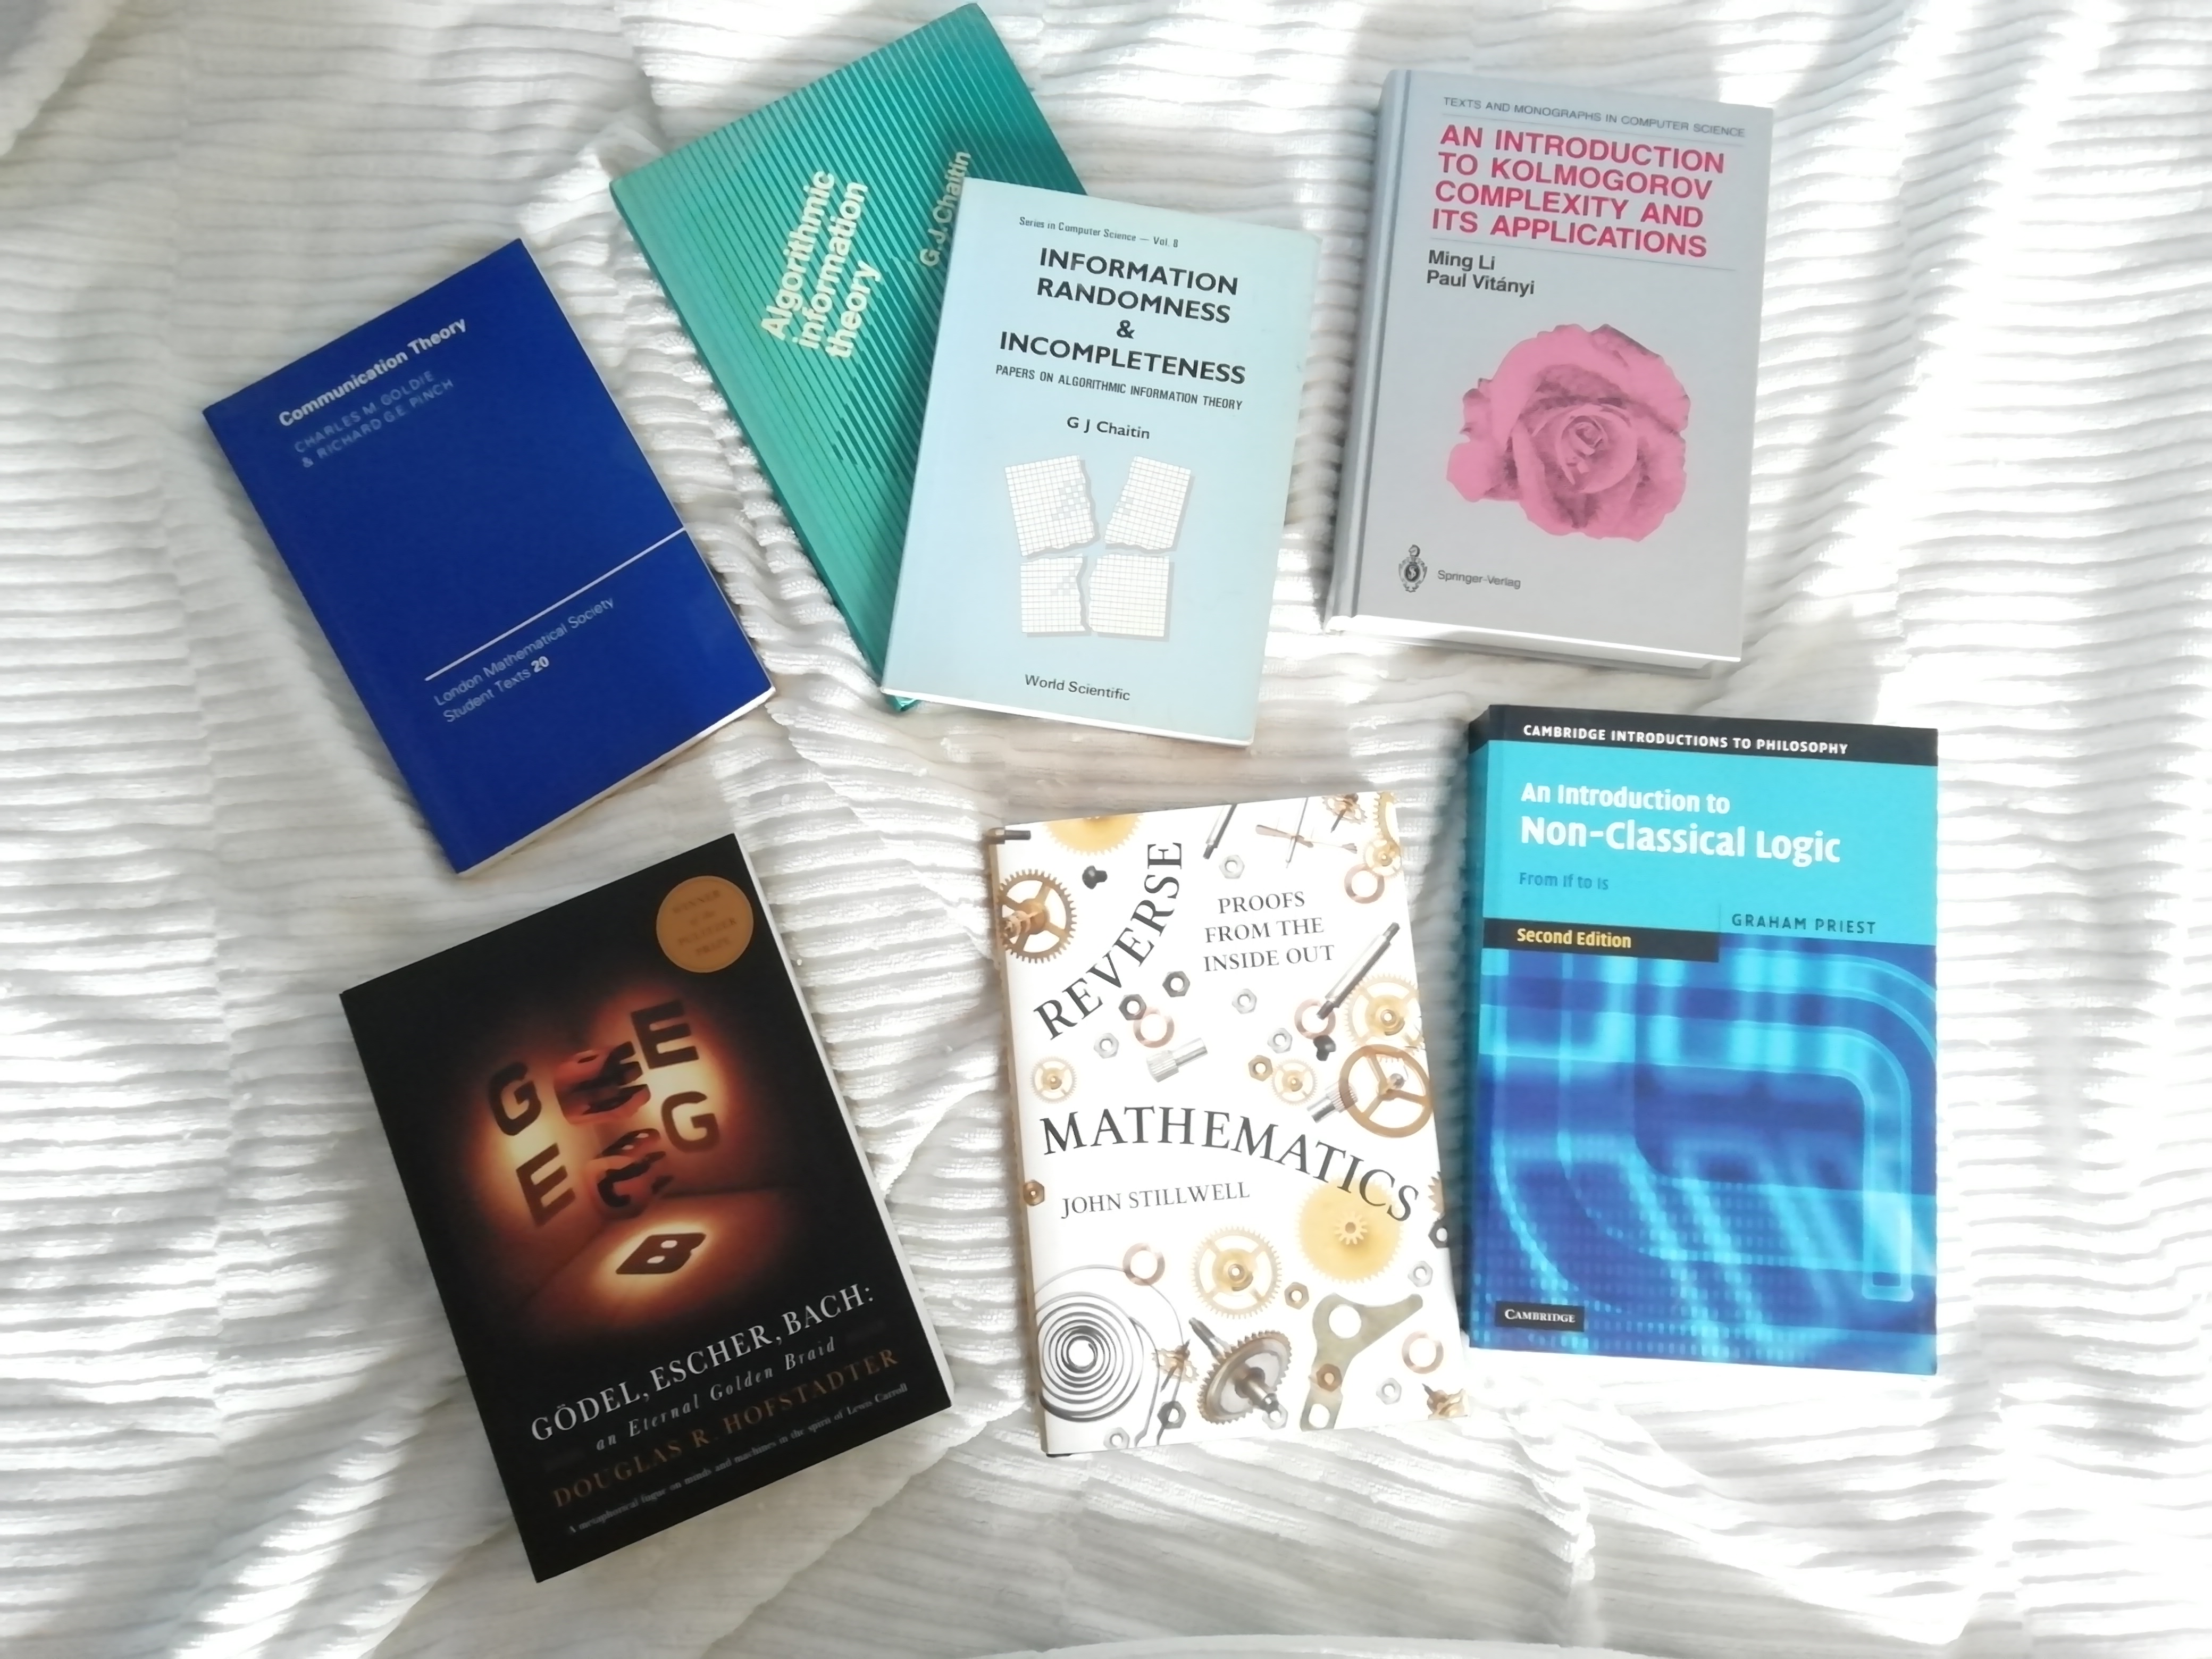
\includegraphics[width=.9\textwidth]{images/books.jpg}
\end{center}
\end{frame}

\begin{frame}
\frametitle{Philosophical Hazards}
\framesubtitle{Side effects of this talk may include}
\begin{itemize}
    \item Indifference
    \item Mild interest
    \item Five stages of grief
    \item Intuitionism
\end{itemize}

\end{frame}

\begin{frame}
    \frametitle{Today's menu}
    \begin{enumerate}
        \item The arithmetic definition of real numbers
        \item Computable numbers
        \item Algorithmically random numbers
    \end{enumerate}
\end{frame}

\begin{frame}
    \frametitle{Peano Axioms (1889)}
    \begin{columns}
        \begin{column}{.75\textwidth}
            \begin{enumerate}
                \item 0 is a natural number
                \item If $n$ is a natural number, its successor $S(n)$ is a natural number
                \item For all $n$, $S(n) \neq 0$
                \item For all $m$, $n$, $S(m) \neq S(n) \Rightarrow m \neq n$
            \end{enumerate}
        \end{column}
        \begin{column}{.25\textwidth}
            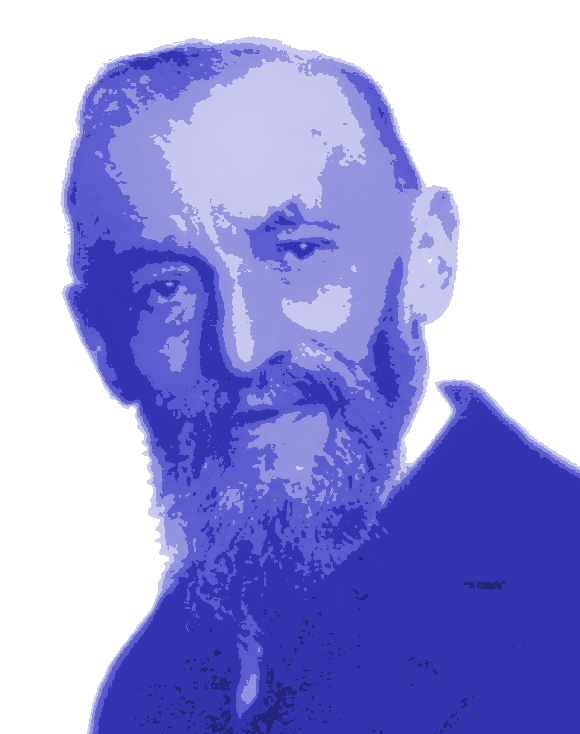
\includegraphics[height=.25\textheight]{images/Giuseppe_Peano.png}
            \vfill
        \end{column}
    \end{columns}
    \vspace{2.5em}
    %\pause[2]
    We call $\N = \{ 0, S(0), S(S(0)), \dots \}$ the set of natural numbers.
\end{frame}

\begin{frame}
    \frametitle{Arithmetic on Peano numbers}
    \framesubtitle{Addition and multiplication are defined recursively}
    For all $m$, $n \in \N$
    \begin{itemize}
        \item $m+0 = m$, and $m+S(n) = S(m+n)$
        \item $m * 0 = 0$, and $m * S(n) = m*n + m$
    \end{itemize}

    \vspace{2.5em}
    $+$ and $*$ are associative and commutative. 

    $*$ is distributive over $+$.
\end{frame}

\begin{frame}
    \frametitle{Integers}
    $$\Z = \{ (m,n) ~|~m,n \in \N \}, $$ 
    where $(m,n)$ is interpreted as $m-n$.

    \vspace{2.5em}
    Relations on $\Z$:
    \begin{itemize}
        \item $(m_1,n_1) = (m_2,n_2) ~\Leftrightarrow m_1 + n_2 = m_2 + n_1$
        \item $(m_1,n_1) < (m_2,n_2) ~\Leftrightarrow m_1 + n_2 < m_2 + n_1$
    \end{itemize}
\end{frame}

\begin{frame}
    \frametitle{Arithmetic on Integers}
    \begin{itemize}
        \item $(m_1,n_1) + (m_2,n_2) = (m_1+m_2, n_1+n_2) $
        \item $(m_1,n_1) * (m_2,n_2) = (m_1*m_2 + n_1*n_2, m_1*n_2 + m_2*n_1)$
        \item $-(m,n) = (n,m)$ (Additive inverse)
    \end{itemize}

    %\pause[2]
    \vspace{2.5em}
    $(\Z, +, *)$ is a \textit{ring}.
\end{frame}

\begin{frame}
    \frametitle{Rationals}
    $$ \Q = \{ (p,q)~| p,q \in \Z, q > 0 \}, $$
    where $(p,q)$ is interpreted as $\frac{p}{q}$.

    \vspace{2.5em}
    Relations on $\Q$
    \begin{itemize}
        \item $(p_1, q_1) = (p_2,q_2) \Leftrightarrow p_1 * q_2 = p_2 * q_1$
        \item $(p_1, q_1) < (p_2,q_2) \Leftrightarrow p_1 * q_2 < p_2 * q_1$
    \end{itemize}
\end{frame}

\begin{frame}
    \frametitle{Arithmetic on Rationals}
    \begin{itemize}
        \item $(p_1,q_1) + (p_2,q_2) = (p_1*q_2 + p_2*q_1, q_1*q_2)$
        \item $(p_1,q_1) * (p_2,q_2) = (p_1*p_2,q_1*q_2)$
        \item $(p,q)^{-1} = (q,p)$ (Multiplicative inverse)
    \end{itemize}

    %\pause[2]
    \vspace{2.5em}
    $(\Q, +, *)$ is a \textit{field}.
\end{frame}

\begin{frame}
    \frametitle{Dedekind cuts}
    \framesubtitle{No relation with the Snyder cut}
    A real number is a set $L \subset \Q$ with an upper bound and such that if $s \in L$ and $t < s$, then $t \in L$, e.g.
    $$ \sqrt{2} = \{ q \in \Q ~|~ q \le 0 \vee q^2 \le 2 \} $$

    \vspace{2.5em}
    Relations on $\R$
    \begin{itemize}
        \item $L_1 = L_2$ (set equality)
        \item $L_1 < L_2 \Leftrightarrow L_1 \subset L_2$
    \end{itemize}

    Arithmetic operations are left as an exercise.
\end{frame}

\begin{frame}
    \frametitle{Computable numbers (Turing 1936)}
    \begin{columns}
        \begin{column}{.75\textwidth}
            A real number $x$ is \textit{computable} if its decimal expansion can be computed to an arbitrary precision using a Turing machine.

            \vspace{2em}
            Equivalently,
            \begin{itemize}
                \item There exists a computable function that, given $\varepsilon >0$, produces a rational $q$ such that $|x-q| < \varepsilon$
                \item The characteristic function of $x$, taken as a Dedekind cut is computable
            \end{itemize}
        \end{column}
        \begin{column}{.25\textwidth}
            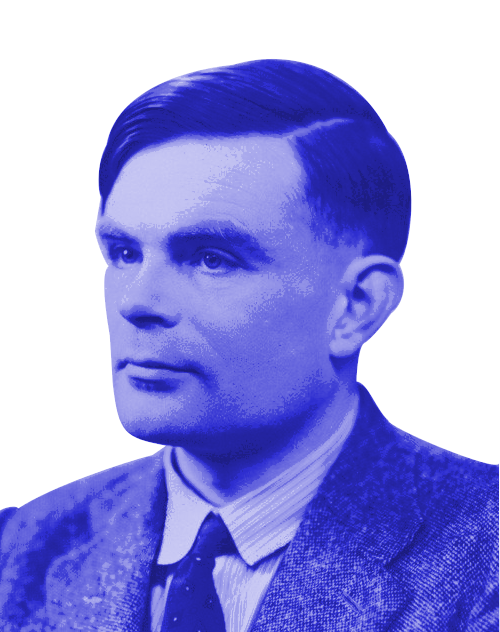
\includegraphics[height=.25\textheight]{images/Turing.png}
            \vfill
        \end{column}
    \end{columns}
\end{frame}

\begin{frame}
    \frametitle{Computable numbers}
    Computable numbers contain
    \begin{itemize}
        \item rational numbers (trivially)
        \item algebraic numbers (by using Newton's method)
        \item $e$, $\pi$
        \item computable functions ($\sin$, $\cos$, $\exp$, \dots) of computable numbers
    \end{itemize}
    
    \vspace{2em}
    However, computable numbers are \textit{countable}!
\end{frame}

\begin{frame}
    \frametitle{Kolmogorov complexity}
    \framesubtitle{aka Program size complexity, algorithmic entropy}
    The Kolmogorov complexity $K_A(s)$ of a sequence $s=(s_1, \dots, s_n)$ in a given language $A$ is the length of the shortest program in $A$ that computes $s$.

    \vspace{2.5em}
    "0101010101010101" $\longrightarrow$ \texttt{"01" * 8}

    "0010100111010101" $\longrightarrow$ \texttt{"0010100111010101"}
\end{frame}

\begin{frame}
    \frametitle{Algorithmically random numbers (Martin-Löf 1966)}
    \begin{columns}
        \begin{column}{.75\textwidth}
            A real number is algorithmically random if the Kolmogorov complexity of its truncated (binary) expansion is "maximal" ($\sim$ diverges)
        \end{column}
        \begin{column}{.25\textwidth}
            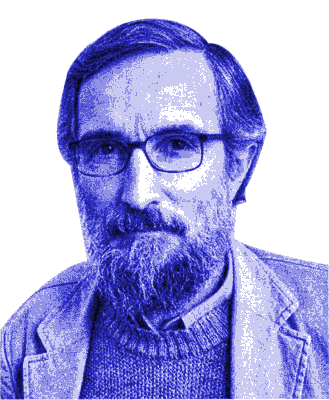
\includegraphics[height=.25\textheight]{images/Per_Martin-Lof.png}
            \vfill
        \end{column}
    \end{columns}
\end{frame}

\begin{frame}
    \frametitle{Properties of ARNs}
    Algorithmically Random Numbers are
    \begin{itemize}
        \item not computable (and vice versa)
        \item incompressible ($\sim$ entropy)
        \item indistinguishable from random noise by any statistical test
    \end{itemize}
    
\end{frame}

\begin{frame}
    \frametitle{Closing thoughts}
    \framesubtitle{Several interesting questions}
    \begin{itemize}
        \item Do non computable real numbers actually exist?
        \item If not, what does it say about the use of real numbers in applied maths?
        \item Is there such a thing as "fundamental randomness", and is it ARNs?
    \end{itemize}
\end{frame}

\begin{frame}
    \begin{center}
        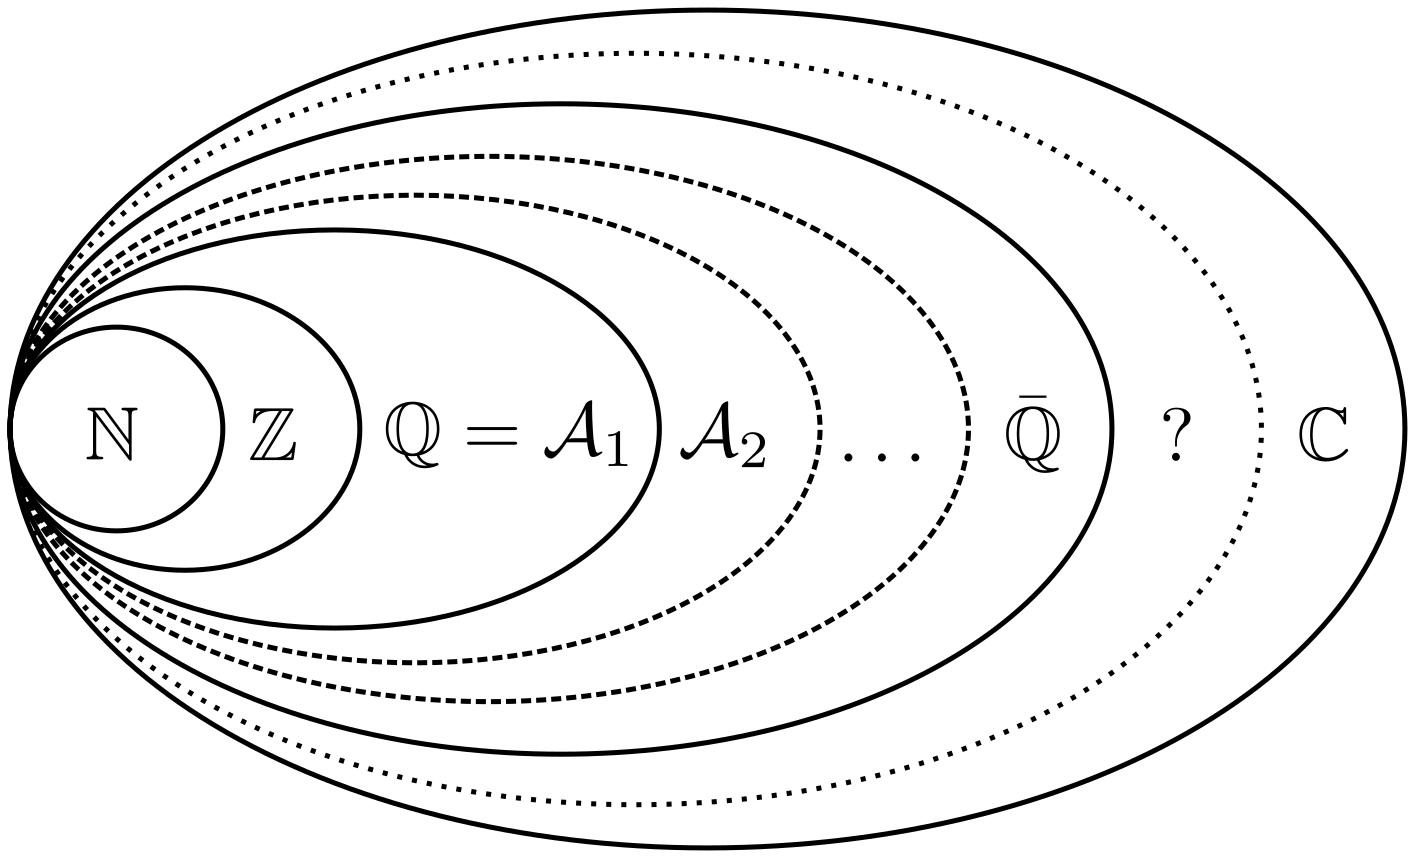
\includegraphics[width=.8\textwidth]{images/numbers.png}
    \end{center}
\end{frame}

\begin{frame}
    \frametitle{That's all folks}
    Slides and references can be found at
    \url{https://github.com/csimal/are-real-numbers-real}
\end{frame}

\end{document}